\chapter{Planificación}

\section{ Planificación inicial}
Se ha realizado una planificación inicial con la fecha objetivo del 14 de Junio del 2018. Se utiliza la herramienta de ``Gantt Project'' para la planificación y se obtiene el diagrama de planificación inicial, ver figura \ref{fig:planificacion_inicial.png}. La planificación está agrupada en varios módulos:\\

\begin{enumerate}
	\item Aprendizaje de la tecnología \textit{Vulkan}. Se destinará una gran cantidad de tiempo para aprender sobre esta nueva tecnología de informática gráfica. Es una tecnología que se liberó el año 2016 (\cite{KhronosReleasesVulkan2016}), es por ello que he destinado gran parte del tiempo a su aprendizaje a un nivel básico.
	
	\item Entorno de trabajo, al ser \textit{Vulkan} una nueva tecnología la instalación de las librerías y configuración de las mismas, está aun muy verde y hay poca información. En tiempo asignado para la correcta configuración y puesta en funcionamiento es de 7 días.
	
	\item Desarrollo de un renderizador. Este modulo cuenta con el desarrollo de una api para mostrar objetos 3D a partir de una malla de triángulos en pantalla. Hay que gestionar la escena, la posición de la cámara y las luces, además de toda la configuración requerida por la API gráfica \textit{Vulkan}. 
	
	\item Modelado de Mallas. La parte de modelación permite seleccionar un vértice del objeto y poder moverlo libremente.
	\item Procesado Geométrico, es la parte principal del trabajo y por tanto para poder aplicar algunos algoritmos se le asigna más tiempo que a ninguna otra tarea.
	
	\item Desarrollo de la memoria. Se va a realizar en paralelo durante todo el proceso de desarrollo de la API.
\end{enumerate}

\begin{figure} %con el [H] le obligamos a situar aquí la figura
	\centering
	\hspace*{-1.6in}
	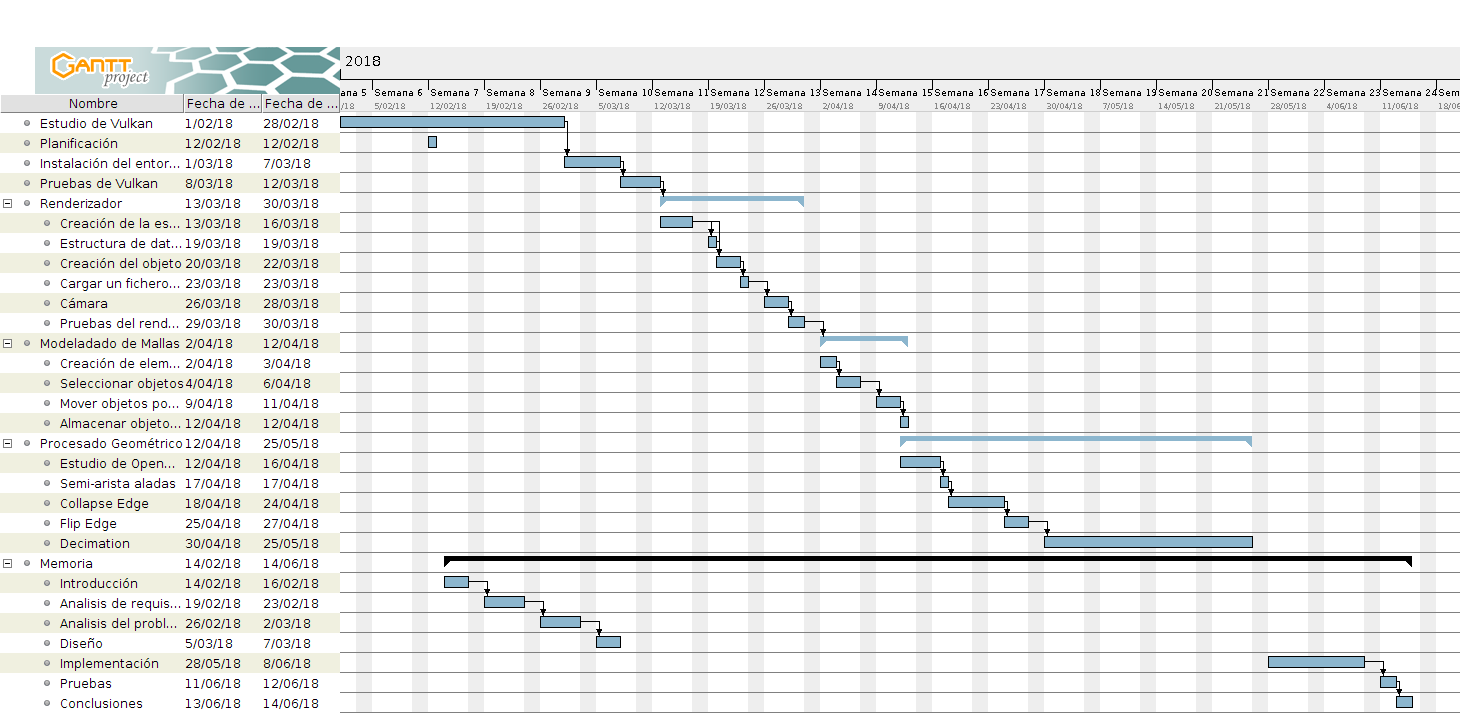
\includegraphics[scale=0.38]{imagenes/Modelator_GP_planning.png} 
	\caption{Diagrama de planificación inicial, por el software ``Gantt Project''} \label{fig:planificacion_inicial.png}
\end{figure}

\subsection{ Avance del proceso}
El trabajo se inició como esta previsto, el primer día de Febrero de 2018, con la documentación y tutoriales de ``Khronos Group'', en \cite{VulkanSubgroupTutorial2018}, \cite{IntroductionVulkanTutorial}, \cite{LunarXchange} la cual es el tutorial oficial que proveé \textit{Khronos Group} para comprobar que funciona correctamente la instalación. Durante el mes de Febrero estuve estudiando el funcionamiento de los buffers, declaraciones y otros elementos a tener en cuenta. Se realizó el trabajo asignado sin problemas durante este periodo.\\

A partir de Marzo empecé con la instalación del entorno en un Sistema Operativo Windows 10 y en otro basado en Linux (Ubuntu 16.04LST, en concreto). Esta parte se componía de la instalación de los IDEs: \texttt{QTCreator 4.5}, Drivers de \texttt{Vulkan} distribuidos por \texttt{``Lunar Xchange''} y instalación de la librería \texttt{OpenMesh}. Además de la correcta visibilidad por parte de las librerías requeridas hacia el compilador. La instalación en ambos sistemas operativos de \texttt{QTCreator} y el driver de \texttt{Vulkan} se hicieron con forme estaba previsto, pero la configuración de las variables de entorno para la correcta compilación del \texttt{Vulkan} no se completó, lo que derivó en un retraso cada vez más grande. Esta parte estaba prevista completarla en una semana por los problemas que suelen dar las instalaciones de elementos relativamente nuevos, pero aun así no se pudo realizar y a principios de Abril se puso el retraso en conocimiento del Tutor para conseguir arreglarlo. Todo el trabajo ya tenía un retraso de un mes, y en Abril tampoco se consiguió que funcionara correctamente por lo que a finales de Abril se decidió cambiar el driver gráfico a OpenGL y volver a re-calcular el proyecto. Por lo que la planificación inicial no se pudo seguir.


\section{ Planificación inicial con OpenGL}
Dado el cambio del driver gráfico de \textit{Vulkan} por \textit{OpenGL} se ha realizado una nueva planificación y re-estructuración de las tareas pero manteniendo el objetivo principal del proyecto quedando como se muestra en la figura \ref{fig:planificacion_final.png} y \ref{fig:planificacion_final2.png}.\\

Ahora en vez de utilizar la tecnología de \textit{Vulkan} usaremos la última versión de \textit{OpenGL 4.5} aprendiendo a controlar y utilizar los \textit{buffers} y demás características propias de esta versión.

\begin{figure} %con el [H] le obligamos a situar aquí la figura
	\centering
	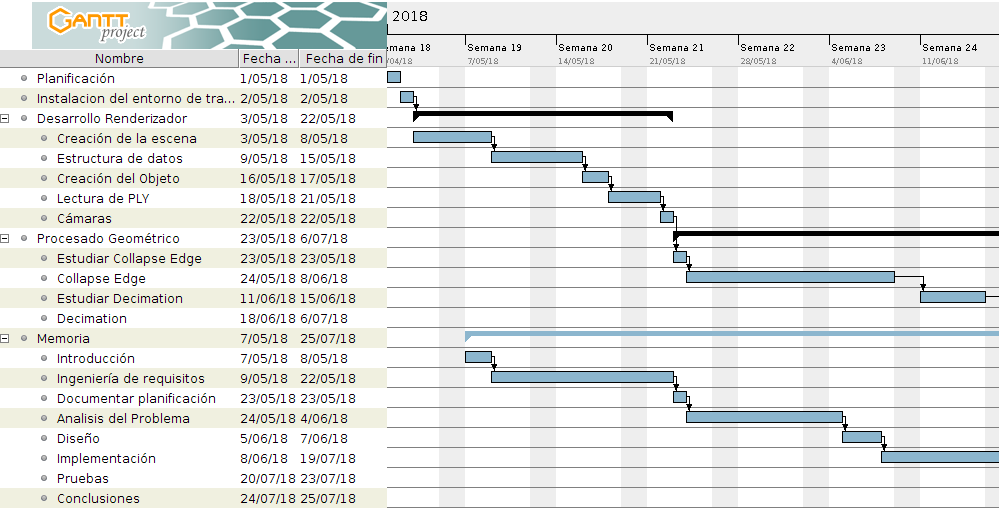
\includegraphics[scale=0.4]{imagenes/Modelator_GP_planning_modi.png} 
	\caption{ (1/2) Diagrama de planificación final, por el software ``Gantt Project''} \label{fig:planificacion_final.png}
\end{figure}

\begin{figure} %con el [H] le obligamos a situar aquí la figura
	\centering
	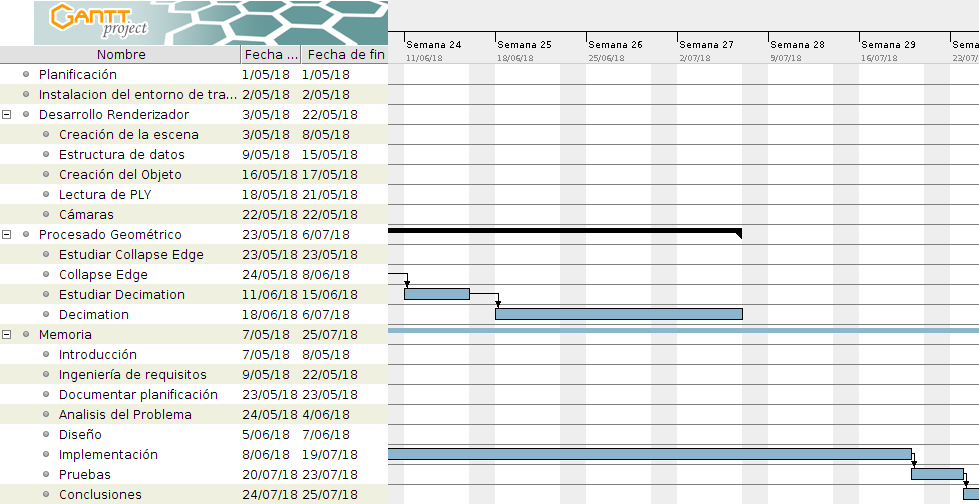
\includegraphics[scale=0.4]{imagenes/Modelator_GP_planning_modi2.png} 
	\caption{ (2/2) Diagrama de planificación final, por el software ``Gantt Project''} \label{fig:planificacion_final2.png}
\end{figure}

\subsection{ Detalle de los procesos}

Los primeros días de mayo se realizó una nueva planificación teniendo en cuenta los nuevos plazos de tiempo y el cambio de driver gráfico resultando de la siguiente forma el progreso.\\

\begin{itemize}
	\item[] \textbf{Planificación (1 de Mayo)}: Se planificó todo el trabajo tareas a realizar sin ningún problema.
	
	\item[] \textbf{Instalación del entorno de trabajo (2 de Mayo)}: Al ser un entorno del que se tiene una base, se realiza en el tiempo establecido.
	
	\item[] \textbf{Desarrollo del Renderizador}: está compuesto por las sub-tareas:
	\begin{enumerate}
		\item \textbf{Creación de la escena (del 3 de Mayo al 8 de Mayo)}: se requiere crear una escena 3D donde poder visualizar y crear los objetos.
		
		\item \textbf{Estructura de datos (del 9 de Mayo al 15 de Mayo)}: Creación de toda la estructura de clases y atributos necesaria para la API, y sus pruebas oportunas.
		
		\item \textbf{Creación del Objeto (del 16 de Mayo al 17 de Mayo)}: Crear un objeto básico y su visualización.
		
		\item \textbf{Lectura de PLY (del 18 de Mayo al 21 de Mayo)}: Poder leer un objeto 3D desde un fichero en formato ``ply'' y almacenarlo en la estructura de datos propia.
		
		\item \textbf{Cámaras (el 22 de Mayo)}: implementación de las cámaras de la escena y su movimiento.
		
	\end{enumerate}
	
	\item[] \textbf{Procesado Geométrico}: estudio e implementación de algoritmos para el procesado geométrico de la malla:
	\begin{enumerate}
		
		\item \textbf{Estudiar Collapse Edge (el 22 de Mayo)}: comprender cómo funciona la operación de colapsar un vértice en otro a través de una semi-arista.
		
		\item \textbf{Collapse Edge (del 24 de Mayo al 8 de Junio)}: implementación del algoritmo de collapse edge y probar que funciona correctamente.
		
		\item \textbf{Estudiar ``Decimation'' (del 11 de Junio al 15 de Junio)}: comprender el funcionamiento del algoritmo para optimizar la malla a través de la eliminación de vértices y aristas del objeto.
		
		\item \textbf{``Decimation'' (del 18 de Junio al 6 de Julio)}: implementación del algoritmo de ``decimation'' y todos los módulos que requiera. Así como su testeo.
	\end{enumerate}

	\item[] \textbf{Memoria}: desarrollo de la memoria del proyecto:
	\begin{enumerate}
		\item \textbf{Introducción (del 7 de Mayo al 8 de Mayo)}: introducción de la memoria y la motivación que tengo para realizar este proyecto.
		
		\item \textbf{Ingeniería de Requisitos (del 9 de Mayo al 22 de Mayo)}: todo el proceso de Ingeniería de Software con respecto al diseño previo que requiere un sistema software así como las necesidades de la aplicación.
		
		\item \textbf{Documentar planificación (el 23 de Mayo)}: documentar cómo se ha realizado la planificación y cuales van a ser las tareas a desarrollar en cada fase y durante cuanto tiempo.
		
		\item \textbf{Análisis del Problema (del 24 de Mayo al 4 de Junio)}: analizar detalladamente el problema que se ha detectado y como se va a solucionar.
		
		\item \textbf{Diseño (del 5 de Junio al 7 de Junio)}: realizar todo el diseño software necesario para la implementación del software.
		
		\item \textbf{Implementación (del 8 de Junio al 19 de Julio)}: detallar el proceso de implementación y cómo están realmente implementado el software.
		
		\item \textbf{Pruebas (del 20 de Julio al 23 de Julio)}: documentar cómo se han realizado las pruebas oportunas y en que consisten.
		
		\item \textbf{Conclusiones (del 25 de Julio al 26 de Julio)}: describir mis propias conclusiones al realizar y terminar el proyecto.
	\end{enumerate}
	
\end{itemize}

\subsection{ Avance del proceso}

\textbf{Instalación del entorno de trabajo:} se ha realizado en el plazo previsto, al ser un entorno ya conocido no aparecen ninguna incidencia.\\

\textbf{Desarrollo del Renderizador:} las primeras tareas se realizaron en tiempo y se consiguió el renderizado de un objeto 3D en menos tiempo del planificado, pero al final de proceso se detecta que no se está utilizando correctamente la API gráfica de OpenGL 4.5 y se procede a cambiarla, lo que provoca que se finalice la tarea el 31 de Mayo.\\

\textbf{Procesado Geométrico:} Se inició el 4 de Junio por el retraso ocasionado por la etapa anterior. En detalle el estudio del \textit{``collapse edge''} se llevo a cabo sin problemas y en el tiempo previsto. Pero la implementación tuvo un problema de diseño base en la implementación de la estructura de datos, y se tuvo que retocar la estructura de datos lo que retraso el trabajo dos días. La estructura no estaba originalmente bien construida para soportar las referencias entre los distintos objetos. El resto de la implementación se llevo a cabo en un día más de lo previsto, por lo que se retrasó el trabajo total de esta parte en casi una semana.\\

La segunda parte del procesado geométrico consistía en el entendimiento y desarrollo de un algoritmo de optimización, ``decimation''. El estudio fue complejo ya que mucha documentación son artículos de revistas científicas con un nivel de abstracción bastante alto. El estudio estaba previsto en 4 días pero al final fueron 6 días. 
Una vez entendido el algoritmo se procedió a su implementación en la estructura desarrollada anteriormente.\\

La implementación del algoritmo se realizó con cautela y probando cada método con una malla pequeña y conocida. Aun así se requirieron dos semanas para su desarrollo, puesto que además había que calcular valores auxiliares como el error generado por eliminar una arista de la malla. Una vez terminado se probó con una malla pequeña y conocida con poca reducción y funcionó, pero cuando se realizo la prueba a una malla de verdad con miles de caras y elementos surgió un problema de memoria dinámica. Este problema ocasiono un retraso de más de una semana hasta que se descubrió cual era el origen y a partir de ahí se procedió a evaluar la mejor forma de solucionarlo. Se decidió optar por cambiar las estructuras base de vectores por listas doblemente enlazadas, por lo que habría que cambiar partes de la estructura de datos. En total se retrasó la tarea dos semanas más de trabajo real. Pero como se pausó el arreglo del fallo para continuar con el desarrollo de la memoria en agosto, se terminó la tarea el 4 de septiembre. \\

\textbf{Desarrollo de la Memoria:}
La memoria se empezó a desarrollar al principio de mayo, el capítulo de introducción e Ingeniería de Requisitos se terminó en el plazo previsto y se mandó a revisión por el tutor. El tutor respondió con los cambios que consideró necesarios y se procedió de inmediato a revisarlos e integrar los que se vieron necesarios. Terminando estos capítulos a finales de mayo.

La documentación de la planificación se realizó en primera instancia planificando los tiempos y las tareas, pero con los problemas surgidos se ha ido completando esta sección con forme se terminaban las tareas implicadas.

El análisis como ya se había realizado fue perfectamente en el tiempo dado, se plasmo las ideas obtenidas durante esta tarea y se realizó una documentación precisa.

El apartado de diseño se quedó más sencillo ya que al ser una API gráfica y contar con un flujo de trabajo con pocas operaciones de procesado pero complejas se optó por realizar el diagrama de clases para mostrar la estructura del sistema y la organización de la arquitectura.

La implementación una vez realizada se documentó sobre como quedaron las clases y objetos y porqué se construyen de esa forma. Esta partes se desarrollo en el tiempo indicado.

Las pruebas y conclusiones dado que se retrasó todo el trabajo de implementación se tuvo que retrasar esta parte también hasta tenerlo todo funcionando al 100\%. Se realizó en menos tiempo del establecido, ocupando solo dos días y terminando así el proyecto antes de la entrega.

